% Ersteller: 	Daniel Wirth
% Software:	TeX-Distribution --> MiKTeX (https://miktex.org/); Editor --> Texmaker (https://www.xm1math.net/texmaker/)
% Literatur:	.bib erstellt mit JabRef (https://www.jabref.org/); %Achtung: bilatex-mode verwenden (preferences) und dann .bib-file erstellen; Engine --> biber
% Der nachfolgende Praxisbericht wurde für das Praxisseminar im Studiengang BEI angefertigt.
%

\documentclass[a4paper, portrait, 12pt]{scrartcl} % Vorgabe TH Nbg
%%%%%%%%%%% Präambel %%%%%%%%%%%

% Standardpakete
%\usepackage[latin1]{inputenc}
\usepackage[T1]{fontenc}
\usepackage[ngerman]{babel}
\usepackage[left=3cm, right=2cm]{geometry} % Vorgabe TH Nbg
\usepackage{graphicx}
\graphicspath{ {../../img/} }
\usepackage{amsmath,amsfonts}
\usepackage{siunitx}
\usepackage{textcomp} % €
\usepackage[dvipsnames]{xcolor}
\usepackage{xspace} % Sorgt dafür, dass Leerzeichen hinter parameterlosen Makros nicht als Makroendezeichen interpretiert werden

% Formatierung etc.: Allgemein
\usepackage{setspace}
\onehalfspacing % Vorgabe TH Nbg
%\spacing{1.X}
\setlength{\parindent}{0pt} % Kein Einzug
\usepackage{afterpage}
\usepackage{lastpage}
\usepackage{fancyhdr} % Für beliebige Kopf- und Fußzeilen
\pagestyle{fancy}
\fancyhf{} % Löscht vorherige Einstellungen - Gesamt
%\fancyhead{} % Löscht voherige Einstellungen
%\fancyfoot{} % Dito
\renewcommand{\headrulewidth}{0 pt} % Keine obere Trennlinie
%\(this)pagestyle{empty} % Keine Seitenzahlen
%\setcounter{page}{n} % Bestimme Seite mit n bezeichnen, nachfolgende ist dann n+1
\rfoot{\thepage\ von \pageref{LastPage}} % Seite x von y; Vorgabe TH Nbg
\usepackage{enumitem}


% Formatierung etc.: Schrift
\usepackage{lmodern} % bessere Fonts
%\usepackage{ulem} % Unterstreichen
\usepackage{relsize} % Schriftgröße relativ festlegen


% Formatierung etc.: Tabellen/Arrays
%\usepackage{tabularx} % "Einfacher Tabllen gestalten"
%\usepackage{adjustbox}
\usepackage{caption} % Beschriftung von Bildern/Tabellen
\usepackage{subcaption} % Analog zu oben
%\setlength{\topsep}{0pt} % Kein xtra Abstand über Tabulator	
%\setlength{\partopsep}{0pt} % Kein xtra Abstand unter Tabulator	


% Hyperlinks und URLs etc.
\usepackage[ 
       colorlinks=true,		%% wenn keine Farbigen Links: = false
    ]{hyperref}
\hypersetup{colorlinks=true, linkcolor=black, urlcolor=MidnightBlue, citecolor=black}
\urlstyle{same}


% Graphiken, Plots, PDFs etc.
%!TEX root = name.tex % Andere .tex-Datei einbinden
\usepackage{pdfpages}
\usepackage{float}
\usepackage{wrapfig}
%\usepackage{pgfplots}
%\pgfplotsset{width=10cm,compat=1.9} % Zweiten Parameter nicht verändern!


% Rechtschreibung bzw. Trennung
%\hyphenchar\font=\string"7F % Nötig für korrekte Silbentrennung!
%\hyphenation{Kom-pli-ziert-es-Wort}
%\hyphenpenalty = XXX
%\tolerance = XXX


% Mathe
%\usepackage{aligned-overset}
%\usepackage{mathabx} %\widehat{•} & \widecheck{}


% "Speziellere" Befehle
%\newcommand{\forceindent}{\leavevmode{\parindent=1.5em\indent}}


% Bibliographie
\usepackage[style=alphabetic, backend=biber]{biblatex}  
\usepackage{csquotes} % Für Anführungszeichen bei Zitaten
\addbibresource{Bibliographie_Projekt_USB_Oszi.bib}
%\usepackage[nohyperlinks, printonlyused]{acronym} % Abkürzungsverzeichnis


\title{Projekt USB-Oszilloskop}
\author{Samuel Oeser, Nicole Sturm, Daniel Wirth}
\date{\today}


%%%%%%%%%%% Main %%%%%%%%%%%
\begin{document}

\setlist{noitemsep}	% no item separation in lists

%%%%%%%%%%% Deckblatt %%%%%%%%%%%
\maketitle
%\thispagestyle{empty}
\pagebreak

%%%%%%%%%%% TOC %%%%%%%%%%%
%\thispagestyle{empty}
\tableofcontents
\pagebreak

%%%%%%%%%%% Abstract / Zusammenfassung %%%%%%%%%%%
\section{Abstract / Zusammenfassung}

\pagebreak

%%%%%%%%%%% Einleitung %%%%%%%%%%%
\section{Einleitung}
Die vorliegende Projektarbeit wurde im Rahmen des Bachelorstudiengangs Elektrotechnik und Informationstechnik an der Fakultät für Elektrotechnik, Feinwerktechnik und Informationstechnik (EFI) der Technischen Hochschule Nürnberg Georg Simon Ohm durchgeführt. Ziel des Projekt-Moduls ist es, den Studierenden die Möglichkeit zu geben, ihr theoretisch erworbenes Wissen in einem praxisnahen, ingenieurwissenschaftlich strukturierten Entwicklungsprojekt anzuwenden. Die Motivation für die Auswahl des Projektthemas lag in der Abbildung des vollständigen Entwicklungsprozesses eines aus Hardware, Firmware und Software bestehenden Gesamtsystems. Auf diese Weise konnten praxisnahe Erfahrungen in allen wesentlichen Entwicklungsdisziplinen gesammelt werden. Darüber hinaus bot das Projekt die Gelegenheit, die grundlegenden Funktionen eines Oszilloskops zu verstehen und im Rahmen eines Prototyps zu realisieren. Ein weiteres wesentliches Auswahlkriterium für das Thema war die klare Unterteilung in abgegrenzte Aufgabenbereiche, sodass die Teammitglieder ihre Aufgaben eigenständig bearbeiten konnten, während gleichzeitig eine Zusammenarbeit im übergeordneten Kontext möglich war.\\

Das zu Beginn definierte Ziel des Projekts war die Entwicklung eines USB-Oszilloskops. Das Gesamtsystem, bestehend aus selbstentwickelter Hardware und einem über Universal Serial Bus (USB) angeschlossenen Computer, soll die Grundfunktionen eines digitalen Speicheroszilloskops (DSO) abbilden. Die Realisierung sollte durch den Einsatz eines Analog-Digital-Umsetzers (ADC) zur Messwerterfassung sowie eines Mikrocontrollers ($\mu$C) als Schnittstelle zwischen der Hardware (ADC-Schaltung) und der Software (Computer) erfolgen.\\

Das Projektteam setzte sich aus drei Studierenden zusammen: Samuel Oeser war verantwortlich für die Entwicklung der Hardware (HW), Daniel Wirth übernahm die Firmware (FW), während Nicole Sturm die Software (SW) einschließlich der grafischen Benutzeroberfläche (GUI) entwickelte. Die Betreuung des Projekts erfolgte durch Prof. Dr. Sven Loquai, der die Studierenden während des gesamten Entwicklungsprozesses begleitete.
\pagebreak

%%%%%%%%%%% Fachliche Grundlagen %%%%%%%%%%%
\section{Fachliche Grundlagen}

\subsection{Allgemeiner Aufbau eines DSOs}
\label{subsec:oscilloscope_func}
Mühl: \cite[Abb. 14.1]{Muehl2020}

\subsection{Leitungsimpedanzanpassung}

\subsection{ADC-Topologien}

\subsection{AAF-Entwurf (Nyquisttheorem)}
\label{subsec:aaf_nyquist}

\subsection{Frequenzkompensierter Spannungsteiler}
Schrüfer: \cite[S. 114ff]{Schruefer2022}
\pagebreak

\subsection{Endliche Zustandsautomaten (Finite State-Machines - FSMs)}
Die Firmware und Software des Projekts sind als synchronisierte Zustandsautomaten implementiert, um einen deterministischen Ablauf der beiden Programme zu gewährleisten.
\subsubsection{Definition und formale Darstellung}
Ein endlicher Automat (EA - engl. Finite State Machine, FSM) ist ein abstraktes Rechenmodell zur Beschreibung von Systemen. Dieser befindet sich in mindestens einem Zustand von einer Zahl endlicher Zustände. Zustandsübergänge (sog. Transitionen) erfolgen durch Eingaben oder das Auftreten von Ereignissen (spezielle Form der Eingabe).\\

Zustände modellieren, was das System gerade tut bzw. in welchem internen ``Modus`` es sich befindet. Ereignisse sorgen für den Wechsel zwischen Zuständen. Übergänge definieren, wie das System im aktuellen Zustand auf ein Ereignis reagiert.

Ein FSM besteht nach \cite[S. 7ff]{Baesig2019} typischerweise aus:
\begin{itemize}
	\item einer Menge von Zuständen $S$,
	\item einem Anfangszustand $s_0$,
	\item einem Eingabe- oder Ereignisalphabet $E$ (Events),
	\item einem Ausgabealphabet $A$,
	\item einer Zustandsübergangsfunktion $\delta :S\times E\rightarrow S$,
	\item einer Ausgabefunktion $\lambda :S\times E\rightarrow A$,
	\item und einer endlichen (evtl. leeren) Menge der Endzustände $F$.
\end{itemize}

Je nach Modellierung kann das Ausgabealphabet und die Ausgabefunktion, sowie die Menge an Endzuständen entfallen.\\

Unterschieden werden folgende Arten von Endlichen Automaten:
\begin{itemize}
	\item \emph{Deterministische Endliche Automaten (DEA)}:\\
	Ein Automat wird als deterministisch bezeichnet, wenn für jede Kombination aus Eingabedaten und aktuellem Zustand eindeutig festgelegt ist, welcher Folgezustand erreicht wird. Das bedeutet, dass sich das \emph{System zu einem bestimmten Zeitpunkt stets in genau einem definierten Zustand} befindet.
	\item \emph{Nichtdeterministische Endliche Automaten (NEA)}:\\
	Bei einem NEA sind für einen bestimmten Zustand und eine Eingabe keine, genau ein oder mehrere mögliche Zustandsübergänge definiert.
\end{itemize}

DEAs sind einfacher als NEAs zu implementieren, wodurch diese in der Praxis häufiger zur Anwendung kommen (vgl. \cite[S. 14]{Baesig2019}). Im Projekt sind die FSMs als DEAs ausgeführt .\\

Eine weitere Aufgliederung von DEAs erfolgt nach der Abhängigkeit der Ausgabe, wenn diese vorhanden ist (vgl. \cite[S. 8f]{Baesig2019}).
\begin{itemize}
	\item Wenn die Ausgabe nur vom aktuellen Zustand abhängt, handelt es sich um einen \emph{Moore-Automaten}.
	\item Wenn die Ausgabe vom aktuellen Zustand \underline{und} der Eingabe abhängt, handelt es sich um einen \emph{Mealy-Automaten}.
\end{itemize}
Im Projekt kommen Moore-Automaten zur Anwendung.

\subsubsection{Modellierung und Darstellung}

Die Darstellung eines Zustandsautomaten erfolgt üblicherweise mit einem \emph{Zustandsdiagramm} (auch Zustandsübergangsdiagramm), einem gerichteten Graph\footnote{ ``Graphen sind ein [...] Konzept, um Objekte und die Beziehung zwischen diesen darzustellen.``\\Quelle: \href{https://www.tu-chemnitz.de/informatik/theoretische-informatik/TI-1/lecture-notes/06-00-graphs.html}{[Link]}}. Die Knoten stellen die Zustände der Menge $S$ dar und die gerichteten Kanten die Zustandsübergänge. Der Startzustand und die Endzustände werden gesondert gekennzeichnet. Eine übliche Darstellung für einen einfachen Moore-Automaten findet sich in \autoref{fig:statediagram_example}a (\emph{sn} sind die Zustände, \emph{xn} sind Eingaben oder Ereignisse und \emph{yn} sind Ausgaben) (vgl. \cite[S. 9]{Baesig2019}).\\

Die Darstellung des Zustandsdiagramms ist auch als Teil der \emph{Unified Modelling Language (UML)}\footnote{aktueller UML-Standard (V2.5.1): \href{https://www.omg.org/spec/UML/2.5.1/About-UML}{[Link]}} festgelegt, welche auch durch internationale Normung festgeschrieben ist. In der Praxis (vor allem beim händischen Entwurf von Zustandsdiagrammen) hat sich aber ein Mischform bewährt, welche auf einige Elemente der UML zurückgreift (siehe \autoref{fig:statediagram_example}b). Es lassen sich beispielsweise auch hierarchische Strukturen integrieren (verschachtelte Zustände).

\begin{figure}[H]
	\centering
    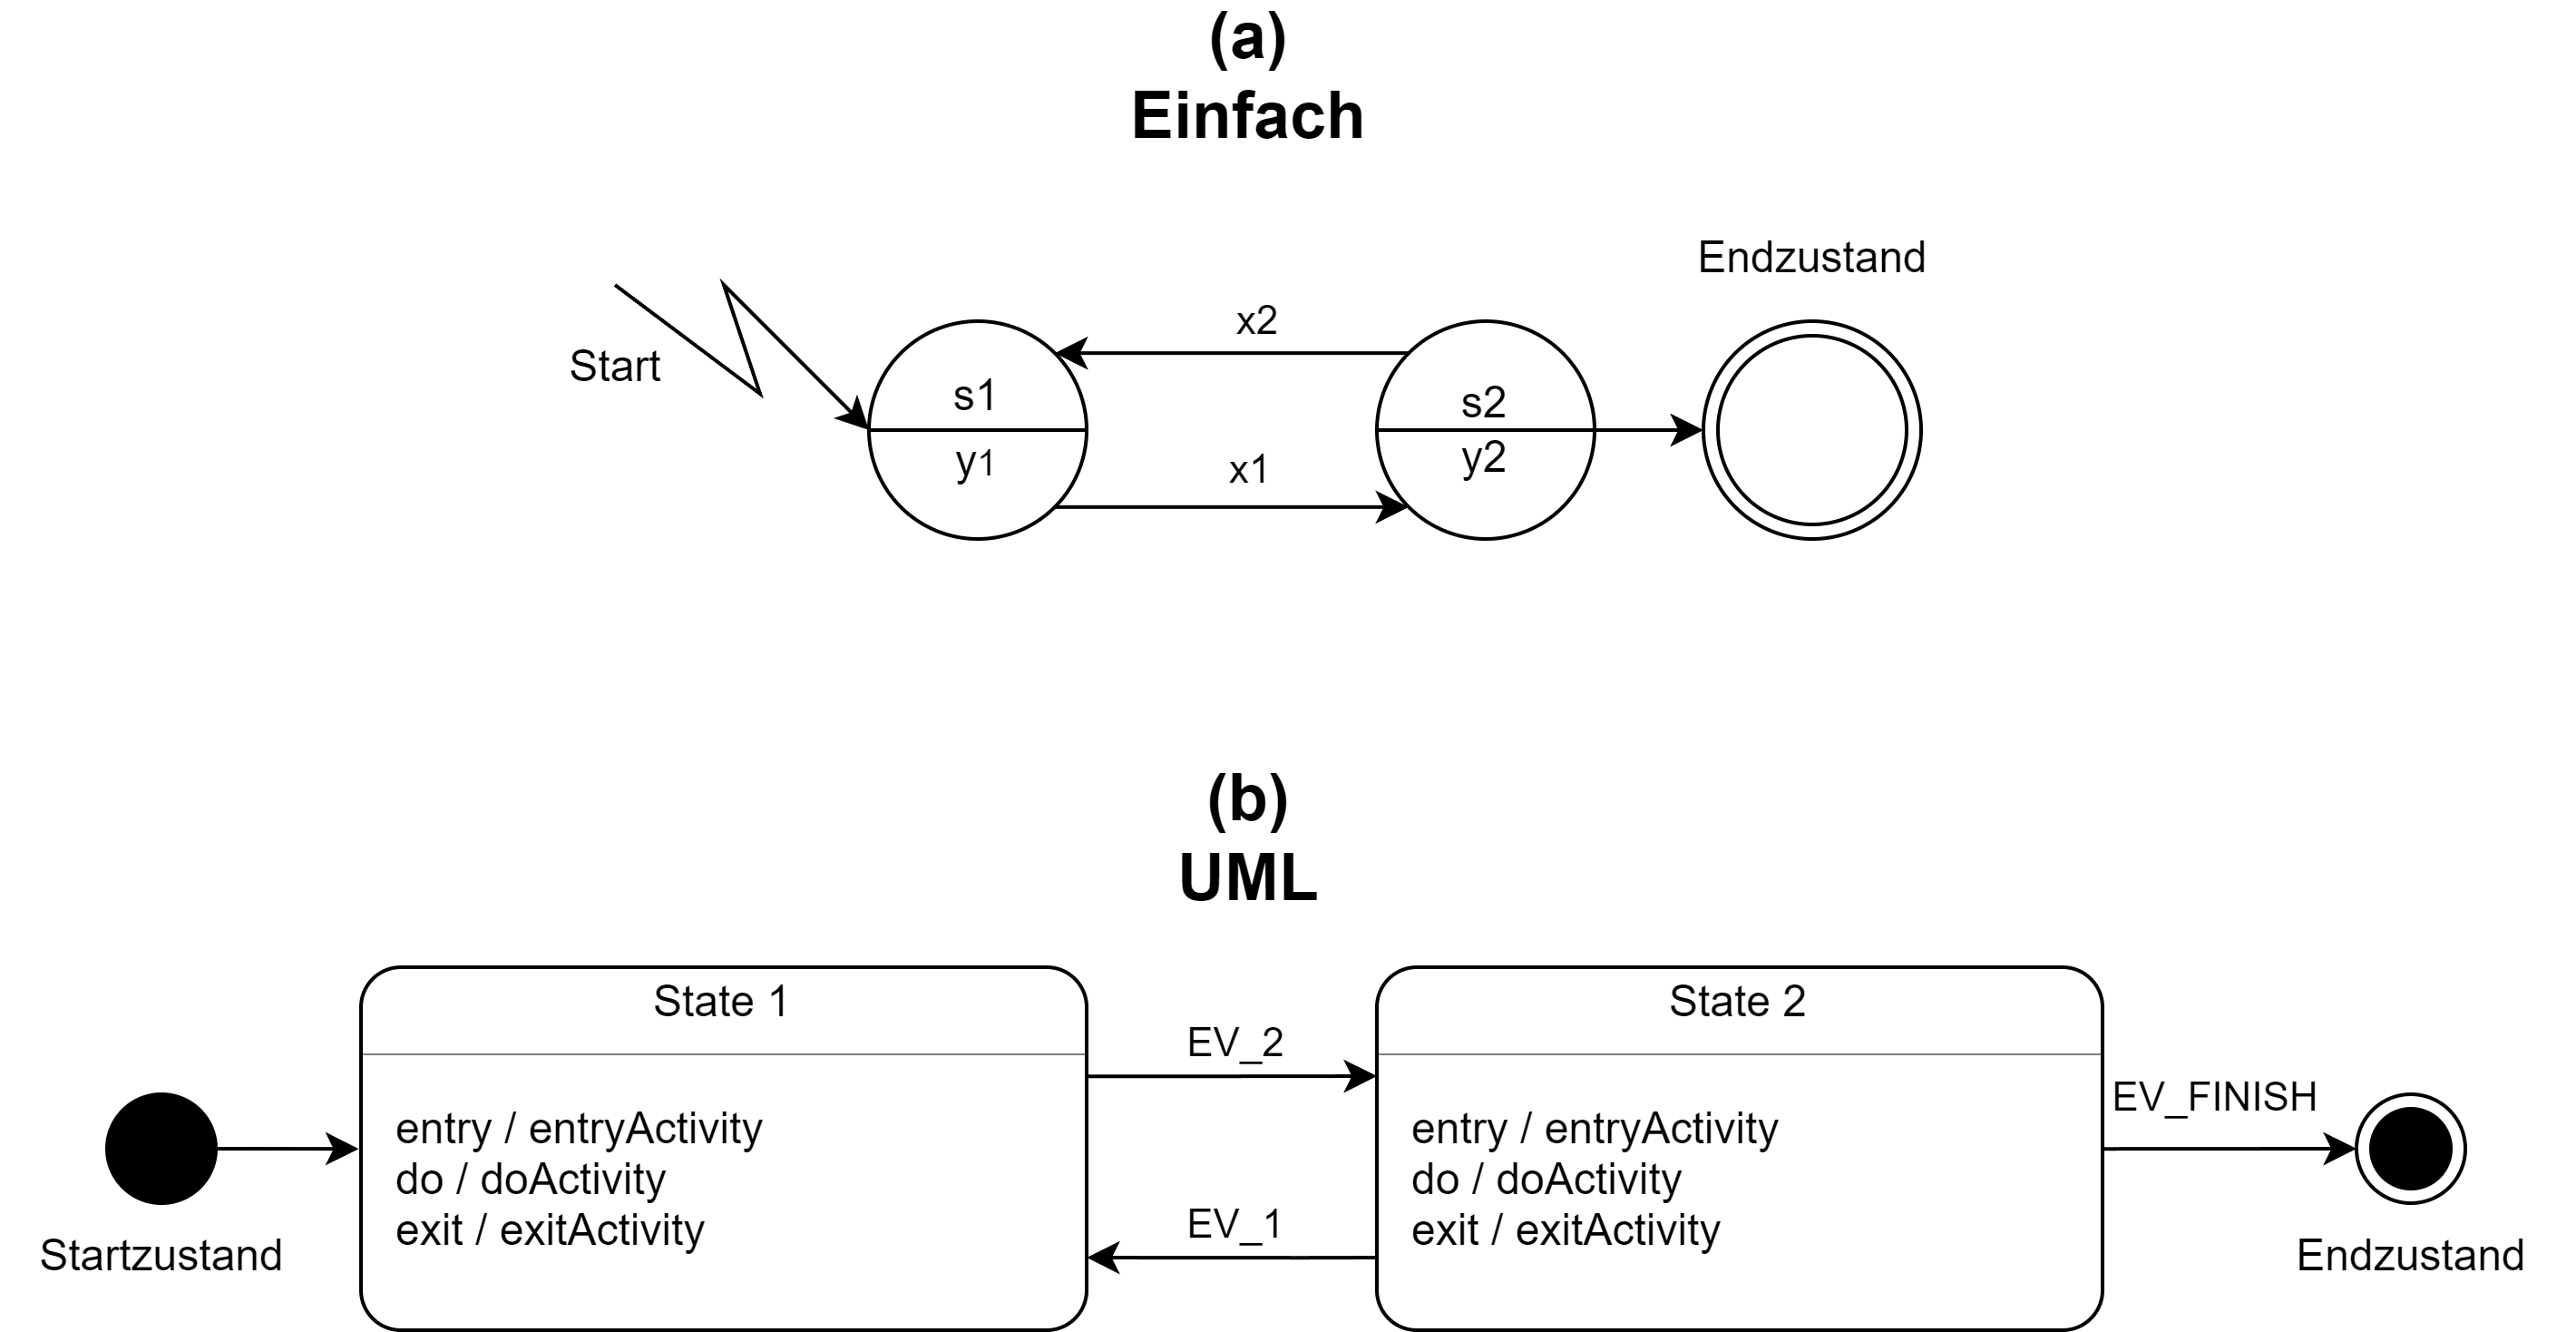
\includegraphics[scale=0.12]{StateDiagram_example.png} 
	\caption{(a) Zustandsdiagramm (nach \cite{Baesig2019}); (b) UML-Zustandsdiagramm}
	\label{fig:statediagram_example}
\end{figure}
\subsubsection{Vorteile einer FSM bei der Programmierung}
\begin{itemize}
	\item \emph{Klarheit \& Übersichtlichkeit}\\
	Der Systemverlauf ist in wohldefinierte Zustände gegliedert. Der Code wird hierdurch verständlicher (kein ``Spaghetti-Code``).
	\item \emph{Deterministisches Verhalten}\\
	Durch die Definitionen, wie auf welches Ereignis reagiert wird, kann die Vorhersagbarkeit und Zuverlässigkeit gewährleistet werden. Außerdem lassen sich undefinierte Zustände durch die explizite Modellierung vermeiden.
	\item \emph{Modularisierung \& Wiederverwendbarkeit}\\
	Einzelne Zustände oder Teile der FSM lassen sich kapseln, segmentieren und wiederverwenden. Teilbereiche können eventuell separat getestet werden.
	\item \emph{Wartbarkeit \& Erweiterbarkeit}\\
	Das System lässt sich durch Hinzufügen neuer Zustände oder neuer Übergänge modular erweitern, ohne die vorhandene Logik stark zu verändern.
	\item \emph{Kommunikation und Dokumentation}\\
	Zustandsdiagramme können bei der Vermittlung von komplexem Programmverhalten gegenüber Nicht-Programmieren genutzt werden.
	\item \emph{Verbessertes Debugging}\\
	Da Zustandsübergänge zentralisiert sind, lassen sich Log-Messages und weitere Debugging-Mechanismen leichter verwenden.
\end{itemize}

\subsection{Direct Memory Access - DMA}
\subsubsection{Allgemeines}
DMA bezeichnet den Vorgang, bei dem durch eine dedizierte Einheit ohne Beteiligung einer CPU Daten transferiert werden (also als Hintergrundprozess). Er kommt zum Einsatz, wenn große Datenmengen von der Peripherie oder einem Speicher zu einem anderen transferiert werden müssen. Ein Chip oder eine Teileinheit eines µC, die solche Transfers durchführt, heißt \emph{Direct Memory Access Controller (DMAC)} (vgl. \cite[S. 125]{Urbanek2020}). Im Folgenden soll die Funktionsweise anhand der Realisierung in der im Projekt verwendeten STM32-Mikrocontrollerfamilie erläutert werden.

\subsubsection{DMA bei STM32-Mikrocontrollern}
Der DMA-Controller ist ein AHB-Modul (AHB - advanced high-performance bus; standardisiertes Bussystem von ARM) und kann wie auch die CPU des Mikrocontrollers (µCs) als Master auf diesen Bus (genauer auf die Bus-Matrix) zugreifen. Durch die Datentransfers, welcher der DMAC nach seiner Konfiguration ohne CPU-Beteiligung ermöglicht, kann die System-Performance deutlich erhöht werden. Die Datentransfers können hierbei per Software oder über angeschlossene Peripherieelemente über sog. \emph{Requests} gestartet werden. Wird als steuerndes Element beispielsweise ein Hardware-Timer genutzt ermöglicht dies die zeitlich exakte Taktung von Datentransfers \cite[S. 6]{STmicroelectronics2016}, was im Projekt für den Abtastvorgang genutzt wird.

\begin{figure}[H]
	\centering
    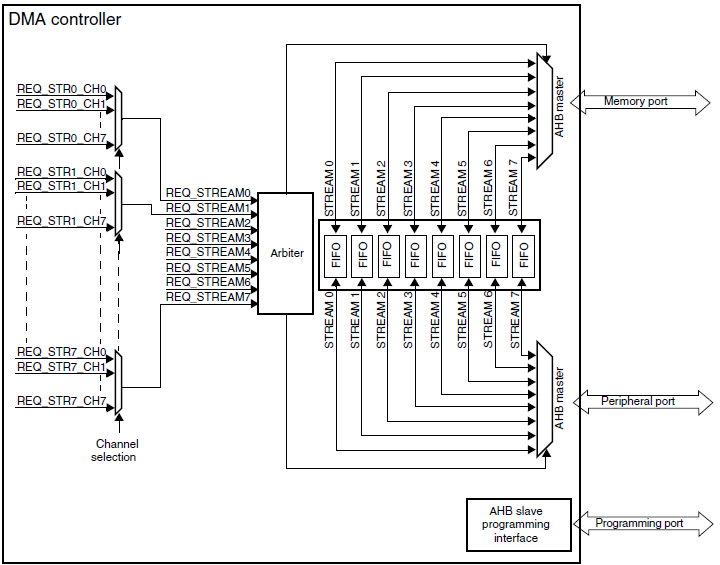
\includegraphics[scale=0.52]{STM32_DMAC.png} 
	\caption{Blockdiagramm STM32-DMA-Controller aus \cite[S. 7]{STmicroelectronics2016}}
	\label{fig:dmac}
\end{figure}

Der µC besitzt zwei unabhängige DMAC, deren Anbindung an Peripherie und Speicher unterschiedlich ausfällt, um alle Ressourcen des Systems flexibel zu verwenden.\\

Der DMAC besitzt 3 Schnittstellen:
\begin{itemize}
	\item \emph{slave port} zur Programmierung des DMAs
	\item \emph{2 master ports} \begin{itemize}
		\item \emph{peripheral port}: peripherieseitiger Datenanschluss
		\item \emph{memory port}: speicherseitiger Datenanschluss
	\end{itemize}
\end{itemize}

Jeder Controller besitzt 8 Datenwege (\emph{Streams}), die separat für unterschiedliche Datentransfers konfiguriert werden können (die Transfers können aber nicht gleichzeitig laufen). Die Streams besitzen hierbei eine konfigurierbare Priorität und ein zentrales Modul, der \emph{Arbiter}, regelt den Zugriff der Streams auf die Ports in Abhängigkeit der Priorität und sorgt für einen deterministischen Ablauf der Transfers. Die einzelnen Streams besitzen noch eine Anzahl an \emph{Channeln}, über die der entsprechende Peripherie-Request für einen Stream ausgewählt werden kann (vgl. \cite[S. 7ff]{STmicroelectronics2016}). Die Zuordnung eines Peripherie-Requests zu einer Channel-Stream-Kombination kann dem Reference-Manual des Controllers entnommen werden (für den STM32F767: \cite[S. 252]{STmicroelectronics2024}).\\

Jeder Stream besitzt außerdem einen 4-stufige \emph{FIFO}-Pufferspeicher (First-In-First-Out), welcher Latenzen beim Zugriff auf das Übertragungsmedium (Bus-Switch-Matrix) überbrücken kann und ein \emph{Verpacken/Entpacken der Daten} erlaubt (z.B.: input: 8bit-Pakete, output: 32bit-Pakete; siehe \autoref{fig:dma_fifo}).

\begin{figure}[H]
	\centering
    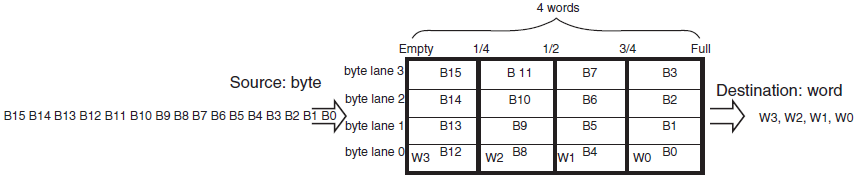
\includegraphics[scale=0.6]{STM32_DMA_FIFO.png} 
	\caption{FIFO-Struktur aus \cite[S. 11]{STmicroelectronics2016} (Teilabbildung)}
	\label{fig:dma_fifo}
\end{figure}
\pagebreak

\textbf{\underline{DMA-Transfers}}\\
Ein Transfer wird zunächst über die \emph{Quelladresse (source address)} und \emph{Zieladresse (destination address)} charakterisiert, hier kann der DMA so konfiguriert werden, dass die Adressen nach einem Transfer automatisch inkrementiert werden können. Somit lassen sich, im Speicher hintereinanderliegende, Daten einfach übertragen. Quell- oder Zeiladresse können jeweils aber auch konstant gehalten werden (siehe späteres Beispiel).

\begin{figure}[H]
	\centering
    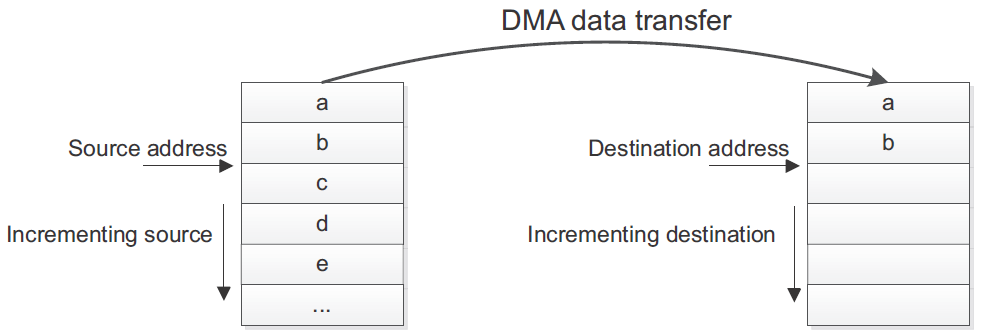
\includegraphics[scale=0.6]{STM32_DMA_transfer_incrementing.png} 
	\caption{DMA Quell- und Zeiladressinkrementierung aus \cite[S. 10]{STmicroelectronics2016}}
	\label{fig:dma_transfer_inc}
\end{figure}

Weitere wichtige Parameter sind die Übertragungsgröße (transfer size), die in einem dedizierten Register (\emph{NDTR} - Number of Data Transfers Register) abgelegt ist, und die Datenbreite (Byte, Half-word, Word). Der Inhalt des NDTR wird nach jedem Transfer entsprechend der Größe des Transfers dekrementiert. Hier wird noch zwischen Circular mode und Normale mode unterschieden. Beim Normal mode ist eine Transaktion (bestehend aus NDTR Transfers) bei NDTR=0 beendet. Der Stream wird deaktiviert und es finden bis zum nächsten Aktivieren des Streams keine Transfers mehr statt. Beim Circular mode wird bei NDTR=0 das Register NDTR mit dem Initialwert geladen und die Transfers beginnen erneut (auch die Adressregister werden mit den Initialwerten geladen) $\rightarrow$ Kreislauf (circular).\\

Die drei möglichen Transfer-Modi sind:
\begin{itemize}
	\item Peripheral-to-Memory (siehe Beispiel in \autoref{fig:periph_to_mem}))
	\item Memory-to-Peripheral
	\item Memory-to-Memory
\end{itemize}

Bei einem Timer-Überlauf des Hardware-Timers TIM1 findet ein DMA-Request statt (ein Stream wurde hierbei entsprechend konfiguriert). Dieser Request löst einen Daten-Transfer zwischen Ziel und Quelle aus (die Datenbreite wurde im Beispiel auf 1 Byte festgelegt). Anschließend werden die Adressen entsprechend der Datenbreite inkrementiert, um die Ziel- und Quelladresse für den nächsten Transfer vorzubereiten. Dieser Prozess geschieht so lange, bis ``Number of Transfers`` durchgeführt worden sind. Der Wert von NDTR wird nach dem Transfer dekrementiert.\\

\begin{figure}[H]
	\centering
    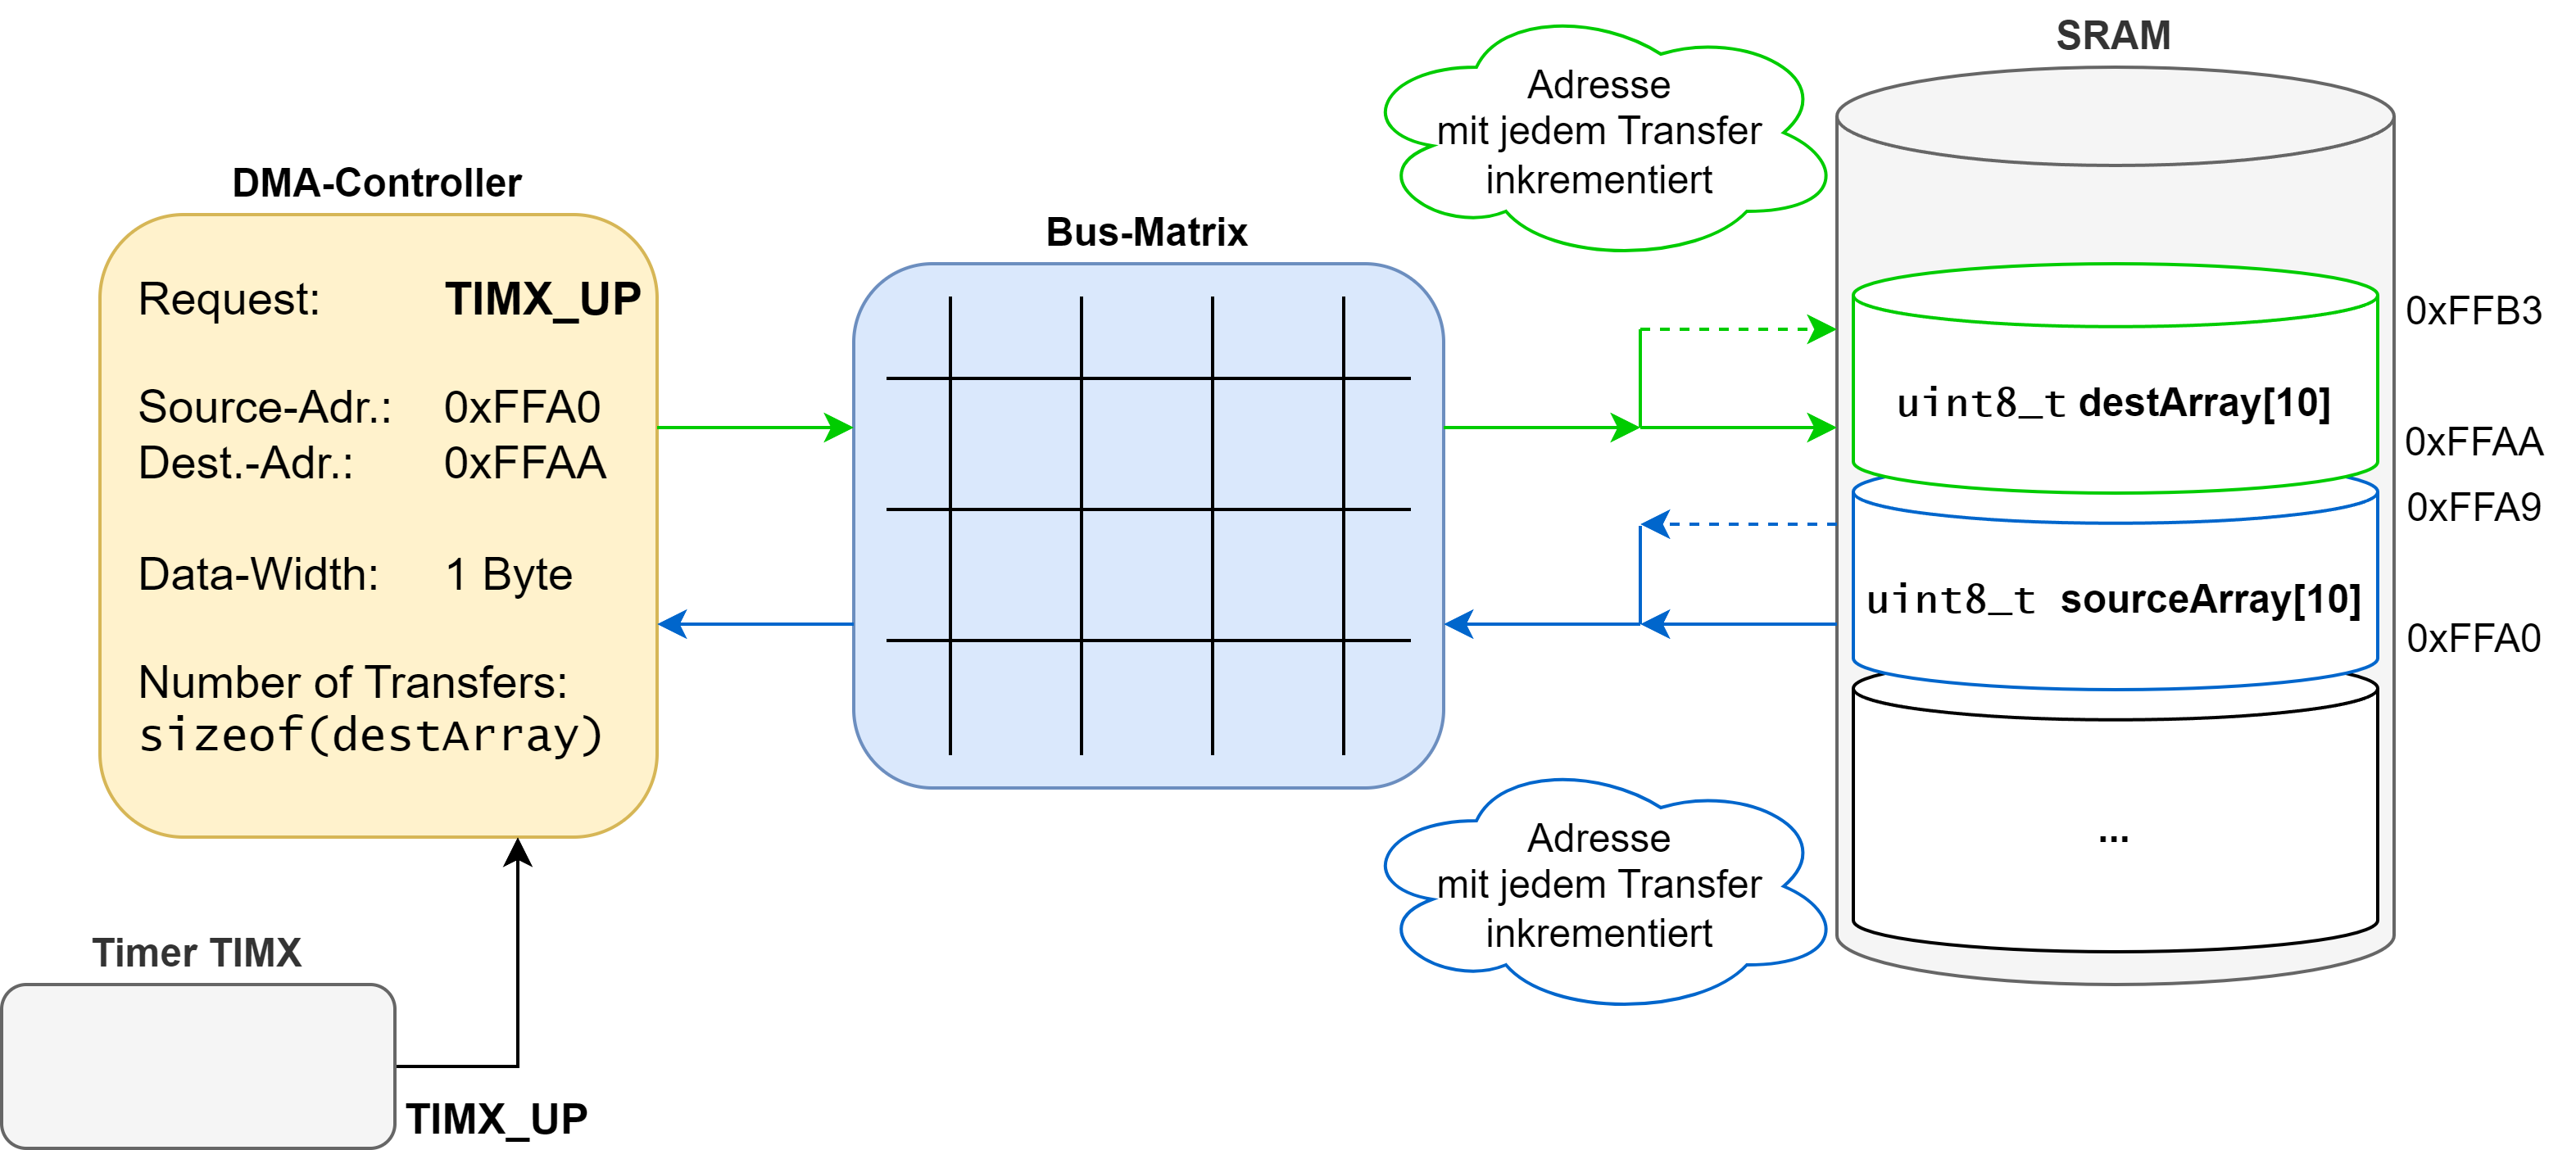
\includegraphics[scale=0.1]{Prinzip_periph2mem.png} 
	\caption{peripheral-to-memory-Transfer}
	\label{fig:periph_to_mem}
\end{figure}

Im Abtastsystem ist keine Inkrementierung der Quelladresse notwendig, da nur das Eingangsdatenregister ausgelesen werden muss, welches die Schnittstelle zum parallelen ADC-Interface darstellt. 

\begin{figure}[H]
	\centering
    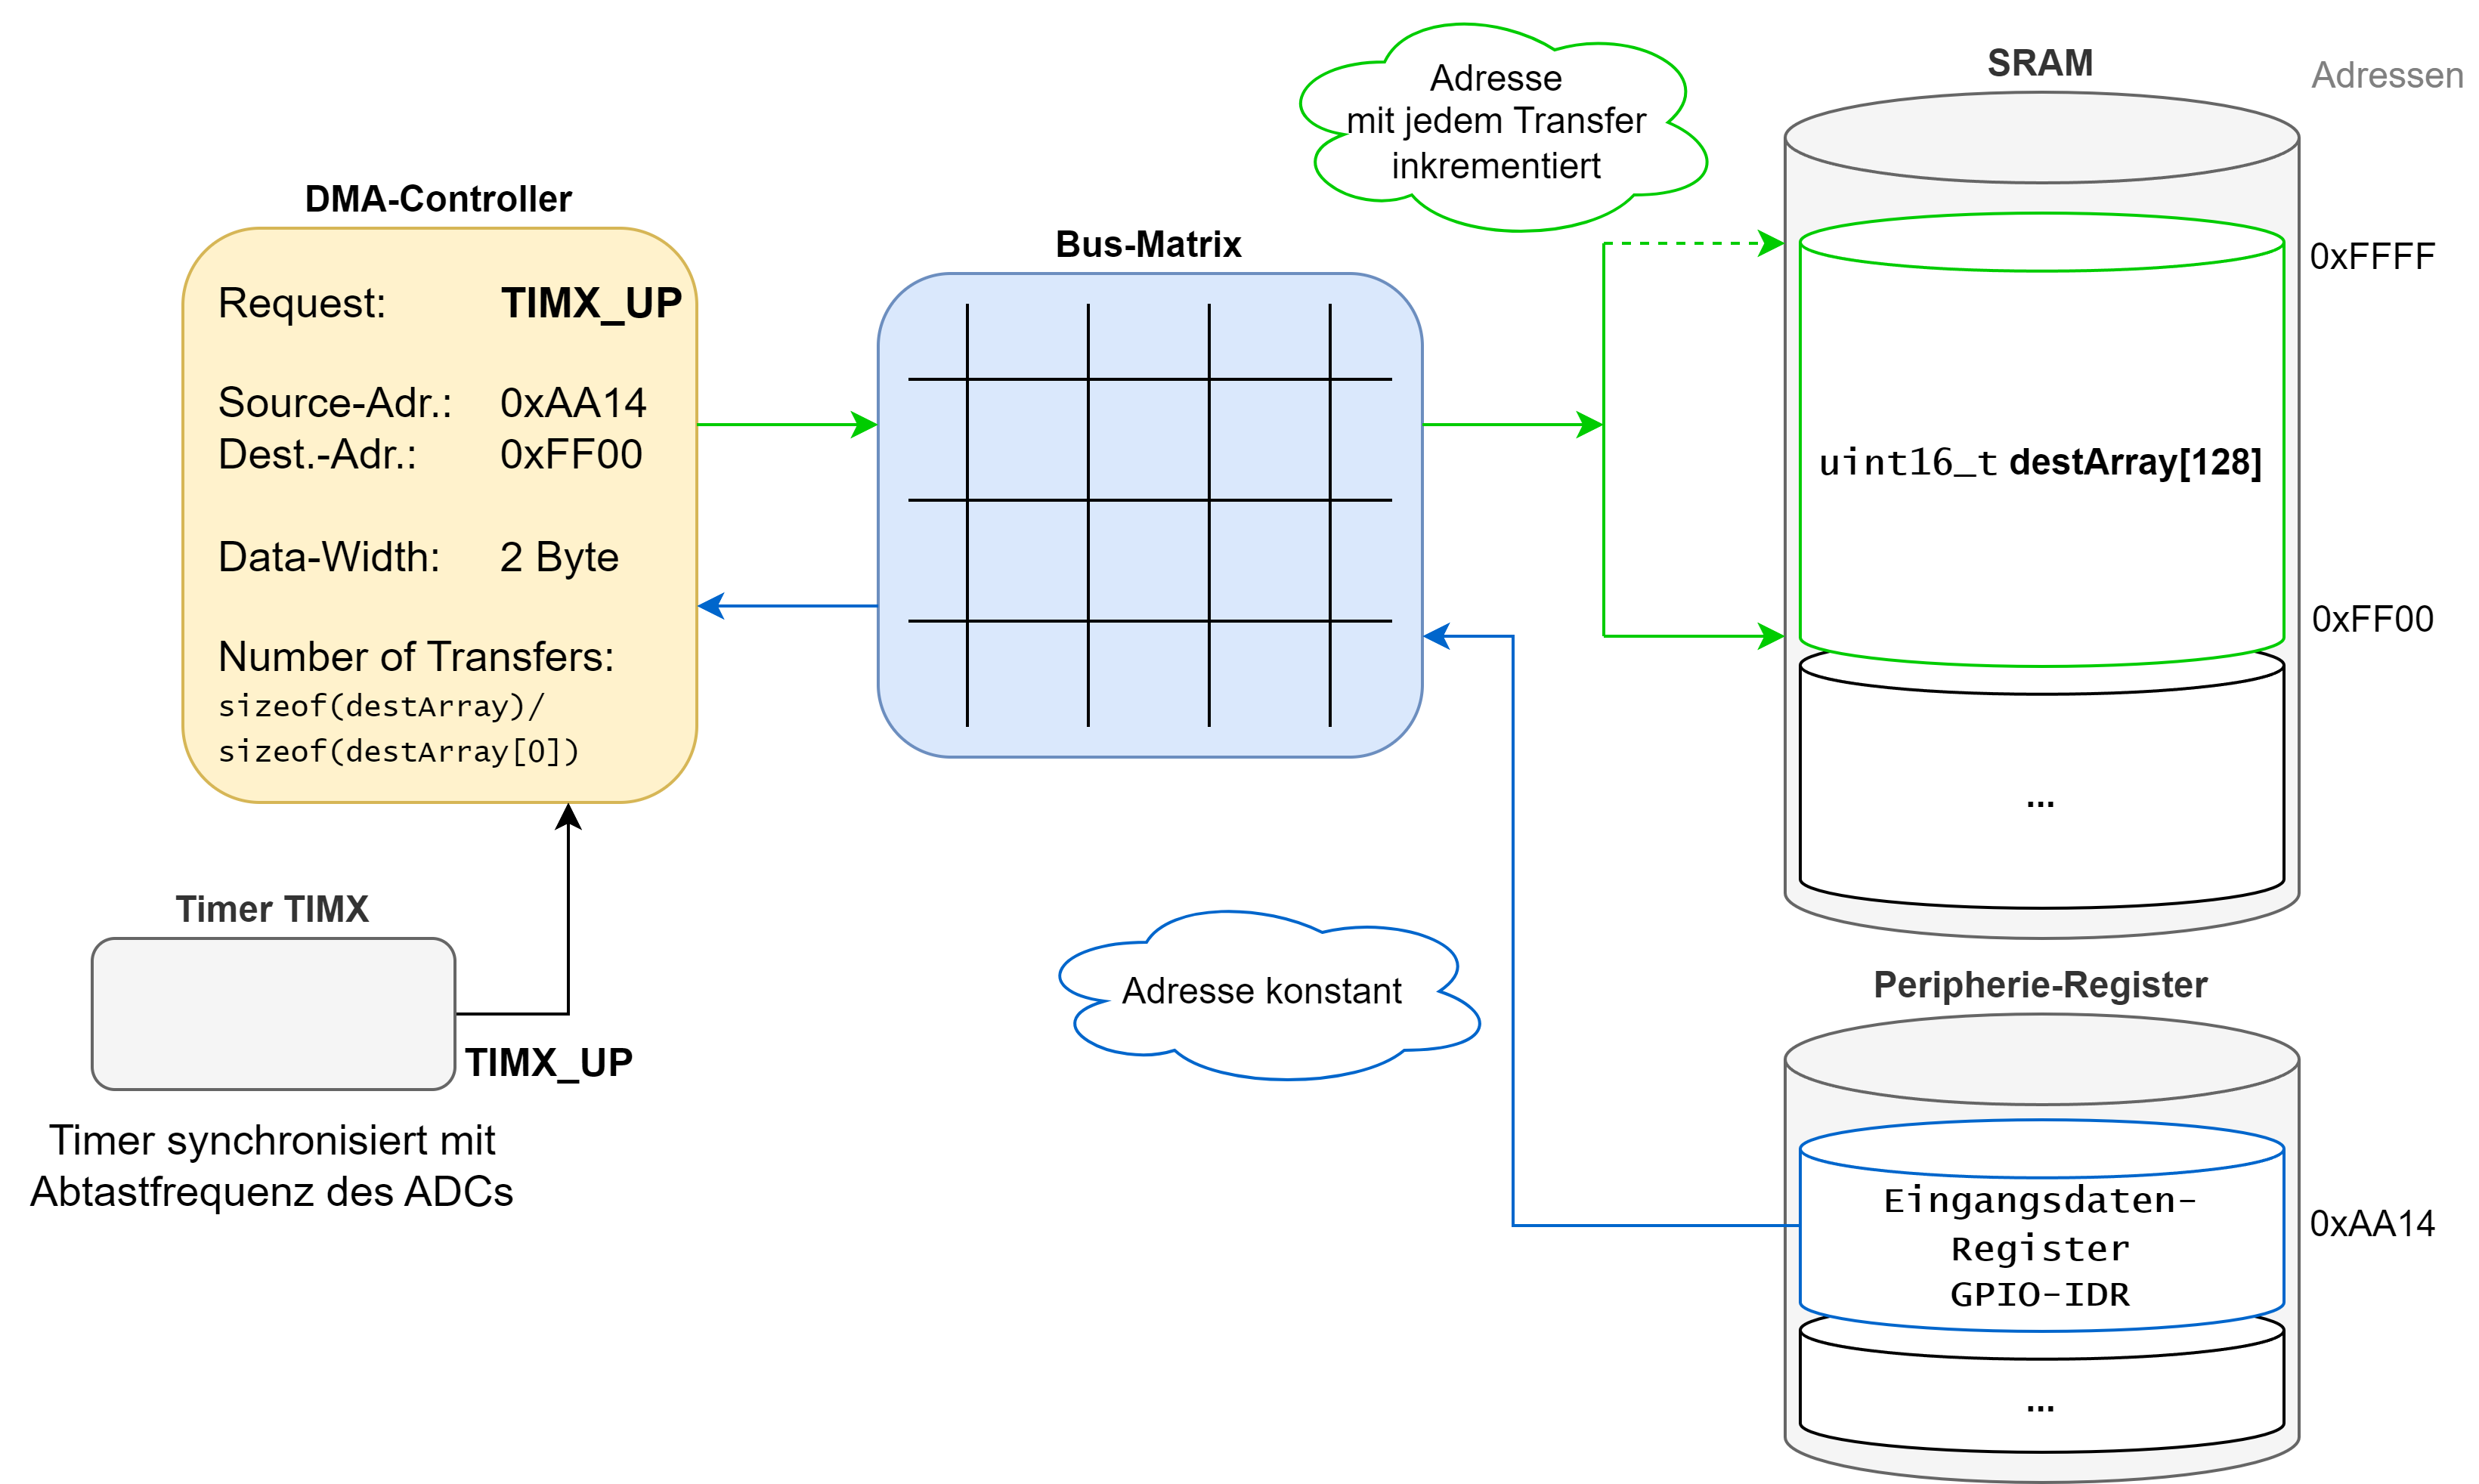
\includegraphics[scale=0.1]{Prinzip_DMA_Datenerfassung.png} 
	\caption{Funktionsprinzip DMA Abtastung}
	\label{fig:periph_to_mem}
\end{figure}

\pagebreak

\textbf{\underline{DMA-Transferwege}}\\

Gemeinsames Übertragungsmedium ist die Bus-Switch-Matrix, die auch in den vorherigen Abbildungen schon dargestellt wurde. Der Zugriff auf diese wird mit Hilfe einer Arbitrierung nach einem round-robin-Algorithmus geregelt. 
Durch den Arbitrierungsvorgang oder die Blockierung des Übertragungsmediums durch einen anderen Bus-Master (z.B. die CPU) kann eine \emph{Latenz beim DMA-Transfer} entstehen.

\begin{figure}[H]
	\centering
    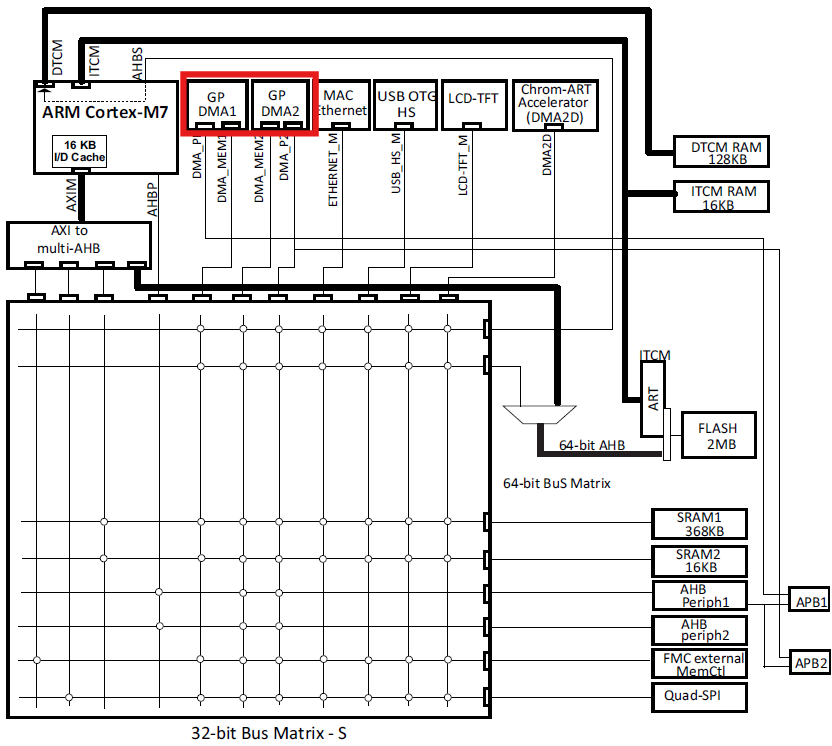
\includegraphics[scale=0.5]{Systemarchitektur_STM32F7.png} 
	\caption{Systemarchitektur für STM32F76xxx $\mu$C aus \cite[S. 72]{STmicroelectronics2024}}
	\label{fig:sysarch_stm32f7}
\end{figure}

Nur Bus-Master (z.B.: Prozessor, DMA-Controller (in \autoref{fig:sysarch_stm32f7} rot hervorgehoben) ) können Lese- und Schreiboperationen initiieren.

\pagebreak

\subsection{Digitale Filterung (Preprocessing)}
\href{https://www.analog.com/en/resources/technical-books/scientist_engineers_guide.html}{The Scientist \& Engineers Guide to Digital Signal Processing, 1999}

\pagebreak

%%%%%%%%%%% Projektkonzeption %%%%%%%%%%%
\section{Projektkonzeption}
\subsection{Vorgehensweise}
Das übergeordnete Vorgehen folgte einem strukturierten Prozess, der sich gut durch das \textbf{V-Modell} visualisieren lässt. Diese Vorgehensweise eignete sich insbesondere aus drei Gründen: \emph{Erstens}, Änderungen an Hardware sind nach deren Umsetzung nur schwer möglich, was iterative Prozesse sehr aufwendig macht. \emph{Zweitens} standen die Projektziele von Beginn an eindeutig fest. \emph{Drittens} waren die Aufgabenbereiche klar voneinander abgegrenzt. Zudem handelte es sich um ein überschaubares Projekt.

\begin{figure}[H]
\centering
    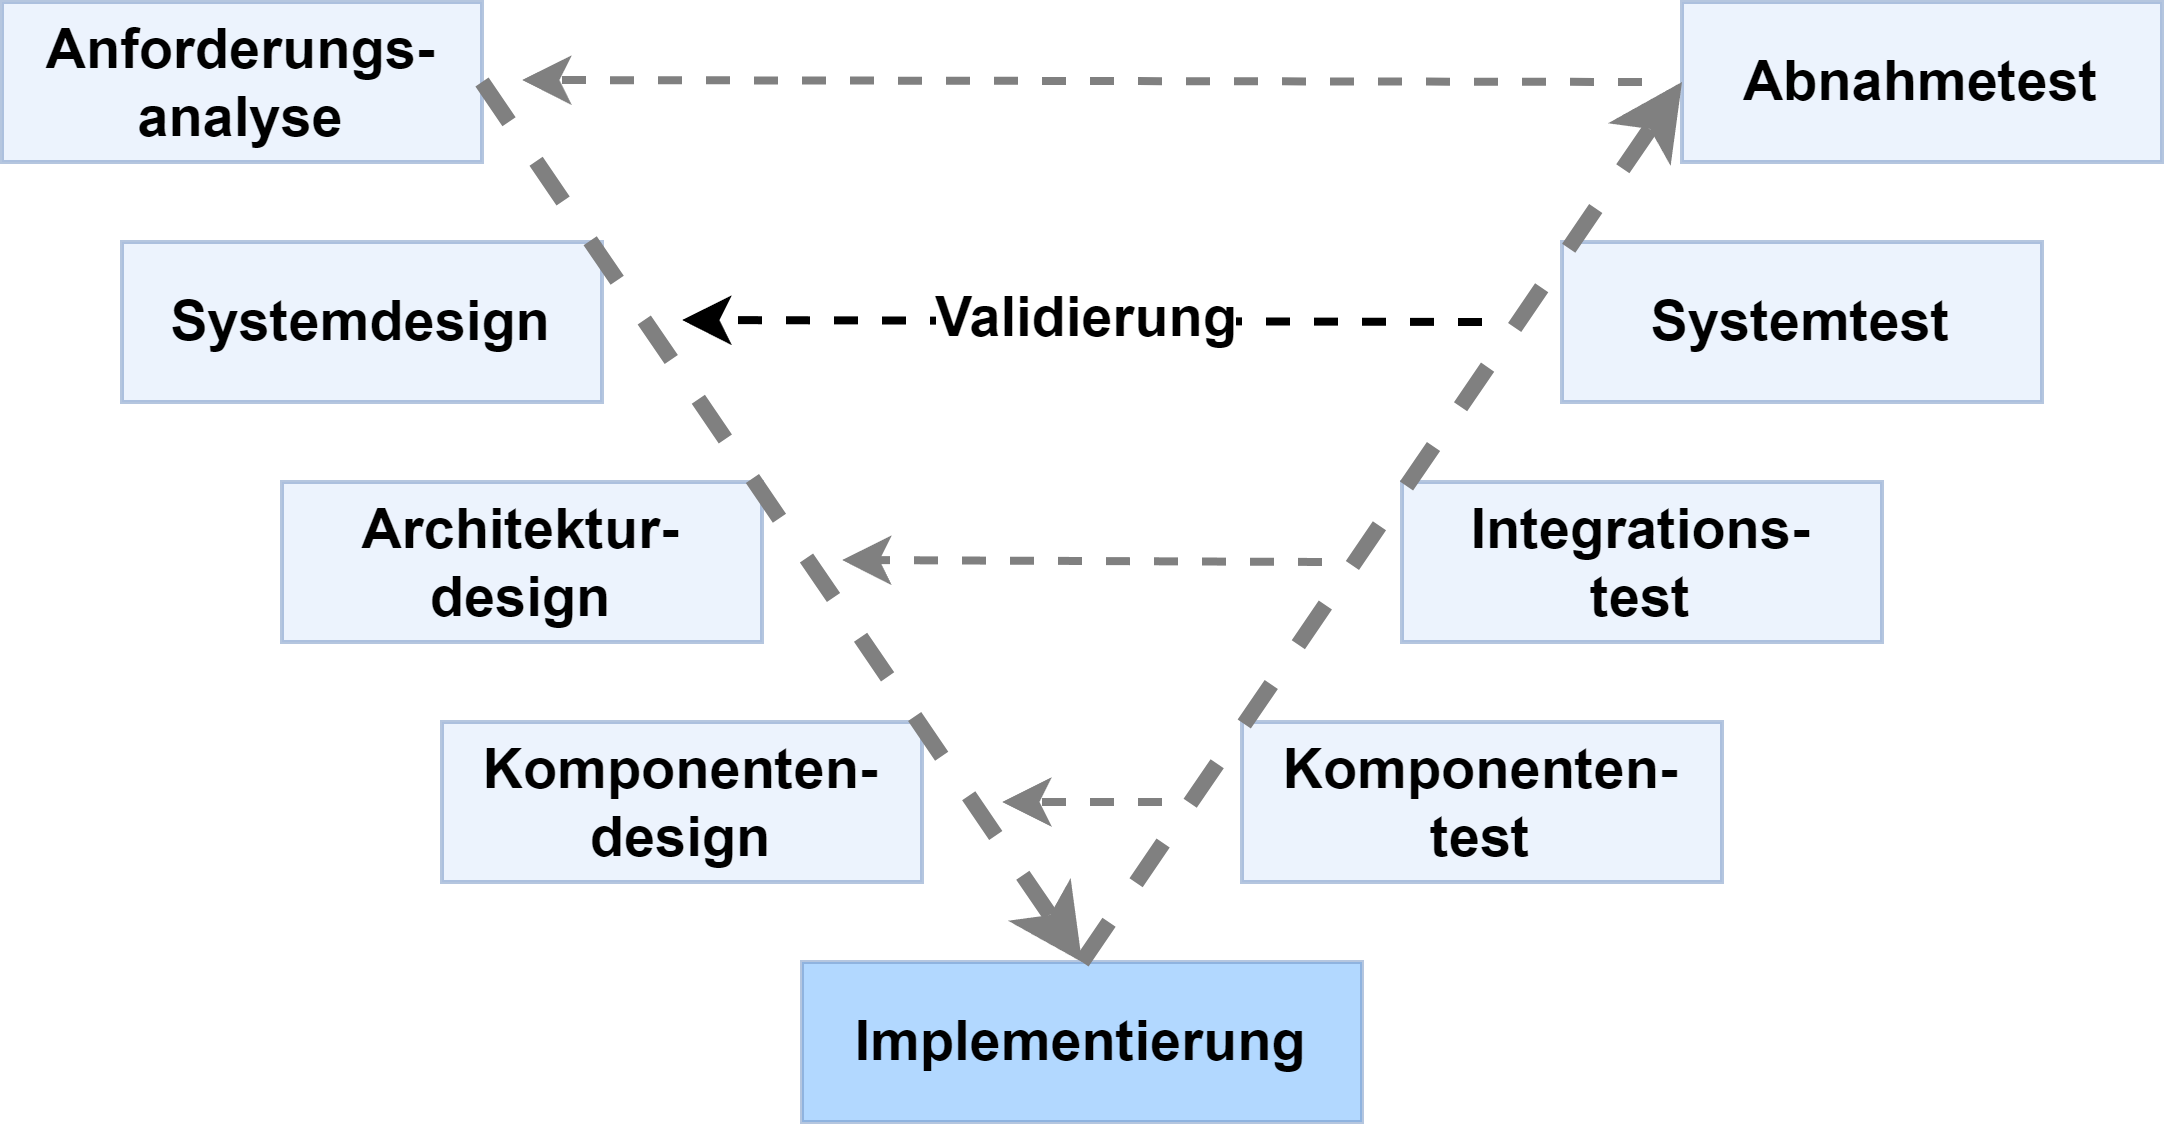
\includegraphics[scale=0.14]{V_Modell.png} 
	\caption{V-Modell}
\end{figure}

Im Folgenden werden die einzelnen Phasen und zugehörigen Validierungsschritte kurz erläutert.\vspace{0.1cm}\\
\underline{Anforderungsanalyse und Abnahmetest}\\
In enger Abstimmung mit dem betreuenden Professor wurden die grundlegenden Anforderungen definiert. Dazu gehörten unter anderem Bandbreite, Abtastrate, Auflösung und Eingangsspannungsbereich. Der spätere Abnahmetest bestand darin zu überprüfen, ob das entwickelte System diese Vorgaben in einer realistischen Versuchsumgebung erfüllte.\vspace{0.1cm}\\
\underline{Systemdesign und Systemtest}\\
Anschließend wurden die grundlegenden Systemfunktionen festgelegt, die zur Erfüllung der Anforderungen notwendig waren. Dazu zählten Signalaufnahme, Digitalisierung, Weiterleitung über USB und Visualisierung am PC. Im Systemtest wurde das fertige Gerät als Gesamtsystem geprüft.\vspace{0.1cm}\\
\underline{Architekturdesign und Integrationstest}\\
In dieser Phase erfolgte die Aufteilung des Systems in die Bereiche Hardware, Firmware und Software. Dabei wurden die Schnittstellen definiert, die ermöglichen sollten, die Module weitgehend unabhängig voneinander zu entwickeln. Diese wurden während des Komponentendesigns bei Bedarf konkretisiert. Im Integrationstest wurde die Zusammenarbeit dieser Module überprüft, insbesondere die zuverlässige Kommunikation zwischen den Subsystemen.\vspace{0.1cm}\\
\underline{Komponentendesign und Komponententest}\\
In dieser Phase wurden die Teilsysteme detailliert ausgearbeitet. Es wurden Konzepte erstellt, Bauteile gewählt, Implementierungsmöglichkeiten abgewogen etc. Jedes Subsystem wurde einzeln getestet, z. B. Spannungsversorgung und ADC in der Hardware, Speicherzugriffe in der Firmware oder Datenanzeige in der Software.\vspace{0.1cm}\\
\underline{Implementierung}\\
In der zentralen Phase wurden die geplanten Komponenten umgesetzt. Dies umfasste das Layout der Schaltungen, die Programmierung der Firmware sowie die Entwicklung der PC-Software. Ziel war es, die entworfenen Module funktionsfähig zu realisieren und für die Integration bereitzustellen.\\

\textbf{Organisation und Zusammenarbeit}\\
Die Zusammenarbeit erfolgte hauptsächlich über ein gemeinsames Projektteam in Microsoft Teams. Dieses war in mehrere Kanäle gegliedert: einen allgemeinen Kanal für projektübergreifende Informationen, jeweils eigene Kanäle für Hardware, Firmware und Software sowie zusätzliche Kanäle für die Schnittstellen. Diese Struktur erleichterte die Ablage von Quellen, Materialien und Informationen und stellte die Übersicht über das gesamte Projekt sicher.\\
Die Abstimmung innerhalb des Teams erfolgte in regelmäßigen Treffen, in denen abgeschlossene Arbeitspakete dokumentiert und neue Zielvorgaben bis zum nächsten Treffen festgelegt wurden. Die Ergebnisse wurden jeweils in Protokollen festgehalten. Eine detaillierte Auflistung der Tätigkeiten sowie deren Zuordnung zu den einzelnen Teammitgliedern findet sich im \nameref{sec:appendix_a} \ref{sec:appendix_a}.
\pagebreak

\subsection{Anforderungen}
Die Anforderungen an das Projekt wurden in Zusammenarbeit mit dem betreuenden Professor sowie dem Laboringenieur des MCT-Labors Hr. Lenkowski nach einer ersten Machbarkeitsanalyse im Hinblick auf die definierten Projektziele festgelegt. Neben den obligatorischen Grundfunktionen eines digitalen Speicheroszilloskops (siehe \autoref{subsec:oscilloscope_func} ``\nameref{subsec:oscilloscope_func}``) wurden folgende zentrale technische Parameter bestimmt:
\begin{itemize}
\item Bandbreite: 1 MHz (Grenzfrequenz des Anti-Aliasing-Filters)
\item Abtastrate: mindestens 10 MS/s (siehe \autoref{subsec:aaf_nyquist})
\item Auflösung: mindestens 10 Bit
\item Analoge Eingangsspannung: ± 5 V
\item Offset: ± 5 V (bezogen auf die Eingangsspannung)
\end{itemize}

Ein weiterer wesentlicher Aspekt war die \emph{Spannungsversorgung} des Systems, für die bewusst keine strikten Anforderungen formuliert wurden. Auf diese Weise sollte während des Entwicklungsprozesses ein höheres Maß an Flexibilität gewährleistet werden, um den Fokus auf die grundlegende Funktionalität des Gesamtsystems legen zu können. Die Signalaufnahme sollte auf \emph{einen Kanal} beschränkt bleiben, um Schwierigkeiten bei der Synchronisation mehrerer ADCs sowie den erhöhten Verwaltungsaufwand für Mehrkanalsysteme zu vermeiden. Außerdem sollte die Möglichkeit bestehen, dass Oszilloskop mit einem Standardtastkopf zu betreiben. Zusätzlich war vorgesehen, die Baugruppe als \emph{erweiterbares Steckboard für ein Mikrocontroller-Entwicklungsboard} umzusetzen, wodurch die Komplexität reduziert und die Funktionalität der Baugruppe in den Vordergrund gestellt werden konnte.\\

Für die Schnittstelle zwischen ADC und Mikrocontroller wurde eine \emph{parallele Anbindung} vorgesehen, da eine serielle Übertragung über SPI bei den geforderten Abtastraten eine zu hohe Taktfrequenz erfordert hätte. Dies hätte einen direkten Datentransfer in den Speicher des Mikrocontrollers nicht mehr zuverlässig ermöglicht. Für die zentrale Recheneinheit wurde sich auf die \emph{Mikrocontroller der STM32-Familie} beschränkt, um vorhandene Kenntnisse aus den Modulen Mikrocomputertechnik und Embedded Systems gezielt einsetzen zu können. Die Kommunikation mit dem PC sollte über eine \emph{USB-Schnittstelle} erfolgen, um eine möglichst uneingeschränkte Kompatibilität zu gewährleisten. Auf dem PC war die Entwicklung einer \emph{eigenen Anwendung zur Visualisierung und Verarbeitung der Messdaten} vorgesehen. Diese sollte über \emph{genormte Kommandos} kommunizieren, sodass auch eine Integration in gängige Entwicklungs- und Analyseumgebungen wie \emph{LabVIEW} oder \emph{MATLAB} möglich wäre.\\

Neben diesen zentralen Vorgaben wurden auch \emph{optionale Erweiterungen} definiert, die nicht als kritisch für den Projekterfolg eingestuft wurden oder den vorgesehenen Arbeitsumfang überschritten. Dazu zählten insbesondere die Implementierung eines \emph{Logikanalysators} mit Protokolldekodierung gängiger Schnittstellen (z. B. SPI, I²C, UART), die Realisierung einer \emph{Fast-Fourier-Transformation (FFT)} zur Spektrumanalyse, die Erweiterung um einen \emph{zweiten analogen Kanal}, die Integration von \emph{Mathematik- und Messfunktionen} sowie die Nutzung unterschiedlicher \emph{Triggerbedingungen}. Weitere Optionen im Hardwarebereich betrafen eine \emph{Optimierung hinsichtlich elektromagnetischer Verträglichkeit (EMV)}, eine \emph{Minimierung des Rauschverhaltens}, die \emph{Stromversorgung über USB} sowie die \emph{Integration des Mikrocontrollers direkt auf der Baugruppe}.

\subsection{Konzept / Architektur}
Parallel zu den Anforderungen wurde ein Konzept entwickelt, um die grundlegende Architektur und Aufgabenverteilung des Projekts festzulegen. Zu Beginn entstand ein grundlegendes, rein funktionales Übersichtsbild (siehe \autoref{fig:block_concept}). Dieses stellt die wesentlichen Signalflüsse und Verarbeitungsschritte dar, die für die Realisierung des USB-Oszilloskops erforderlich sind. Der Signalpfad führt dabei vom Device under Test (DUT) über die Signalerfassung zur Speicherung der Rohdaten und weiter zur Verarbeitung auf PC-Ebene. Dieses Schema diente als Orientierungshilfe für die weiteren konzeptionellen Schritte, ohne jedoch bereits konkrete Funktionseinheiten Bauteile oder Schnittstellen festzulegen.\\

Auf Basis dieser funktionalen Skizze sowie des in der Fachliteratur beschriebenen Grundaufbaus eines digitalen Speicheroszilloskops (siehe \autoref{subsec:oscilloscope_func}) wurde schließlich ein Gesamtkonzept entwickelt, das Funktionseinheiten definiert und den jeweiligen Bereichen Hardware, Firmware und Software zuordnet (siehe \autoref{fig:complete_concept}).

\begin{figure}[H]
	\centering
    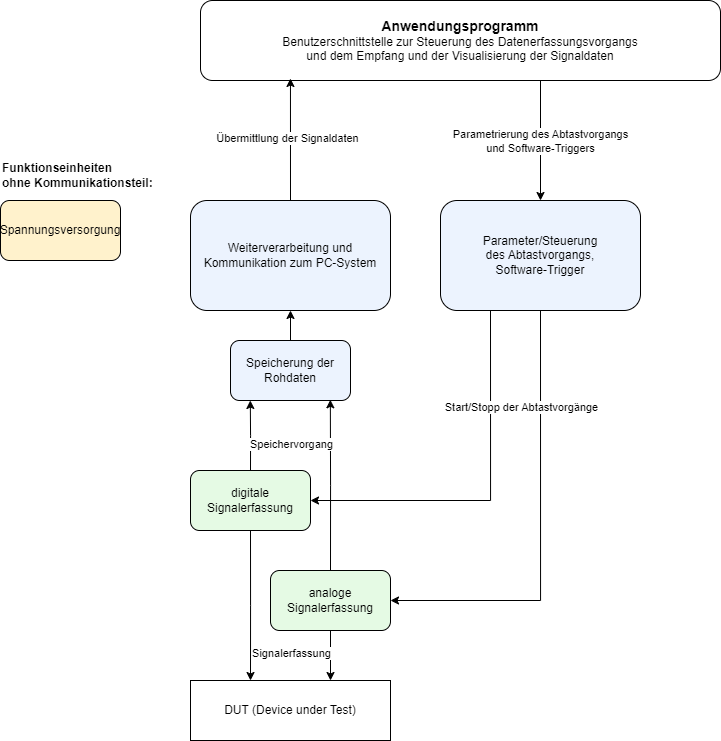
\includegraphics[scale=0.4]{Projektarbeit_Architektur.png} 
	\caption{Übersichts-Blockschaltbild (erstellt für die Konzeptvorstellung)}
	\label{fig:block_concept}
\end{figure}

\begin{figure}[H]
	\centering
    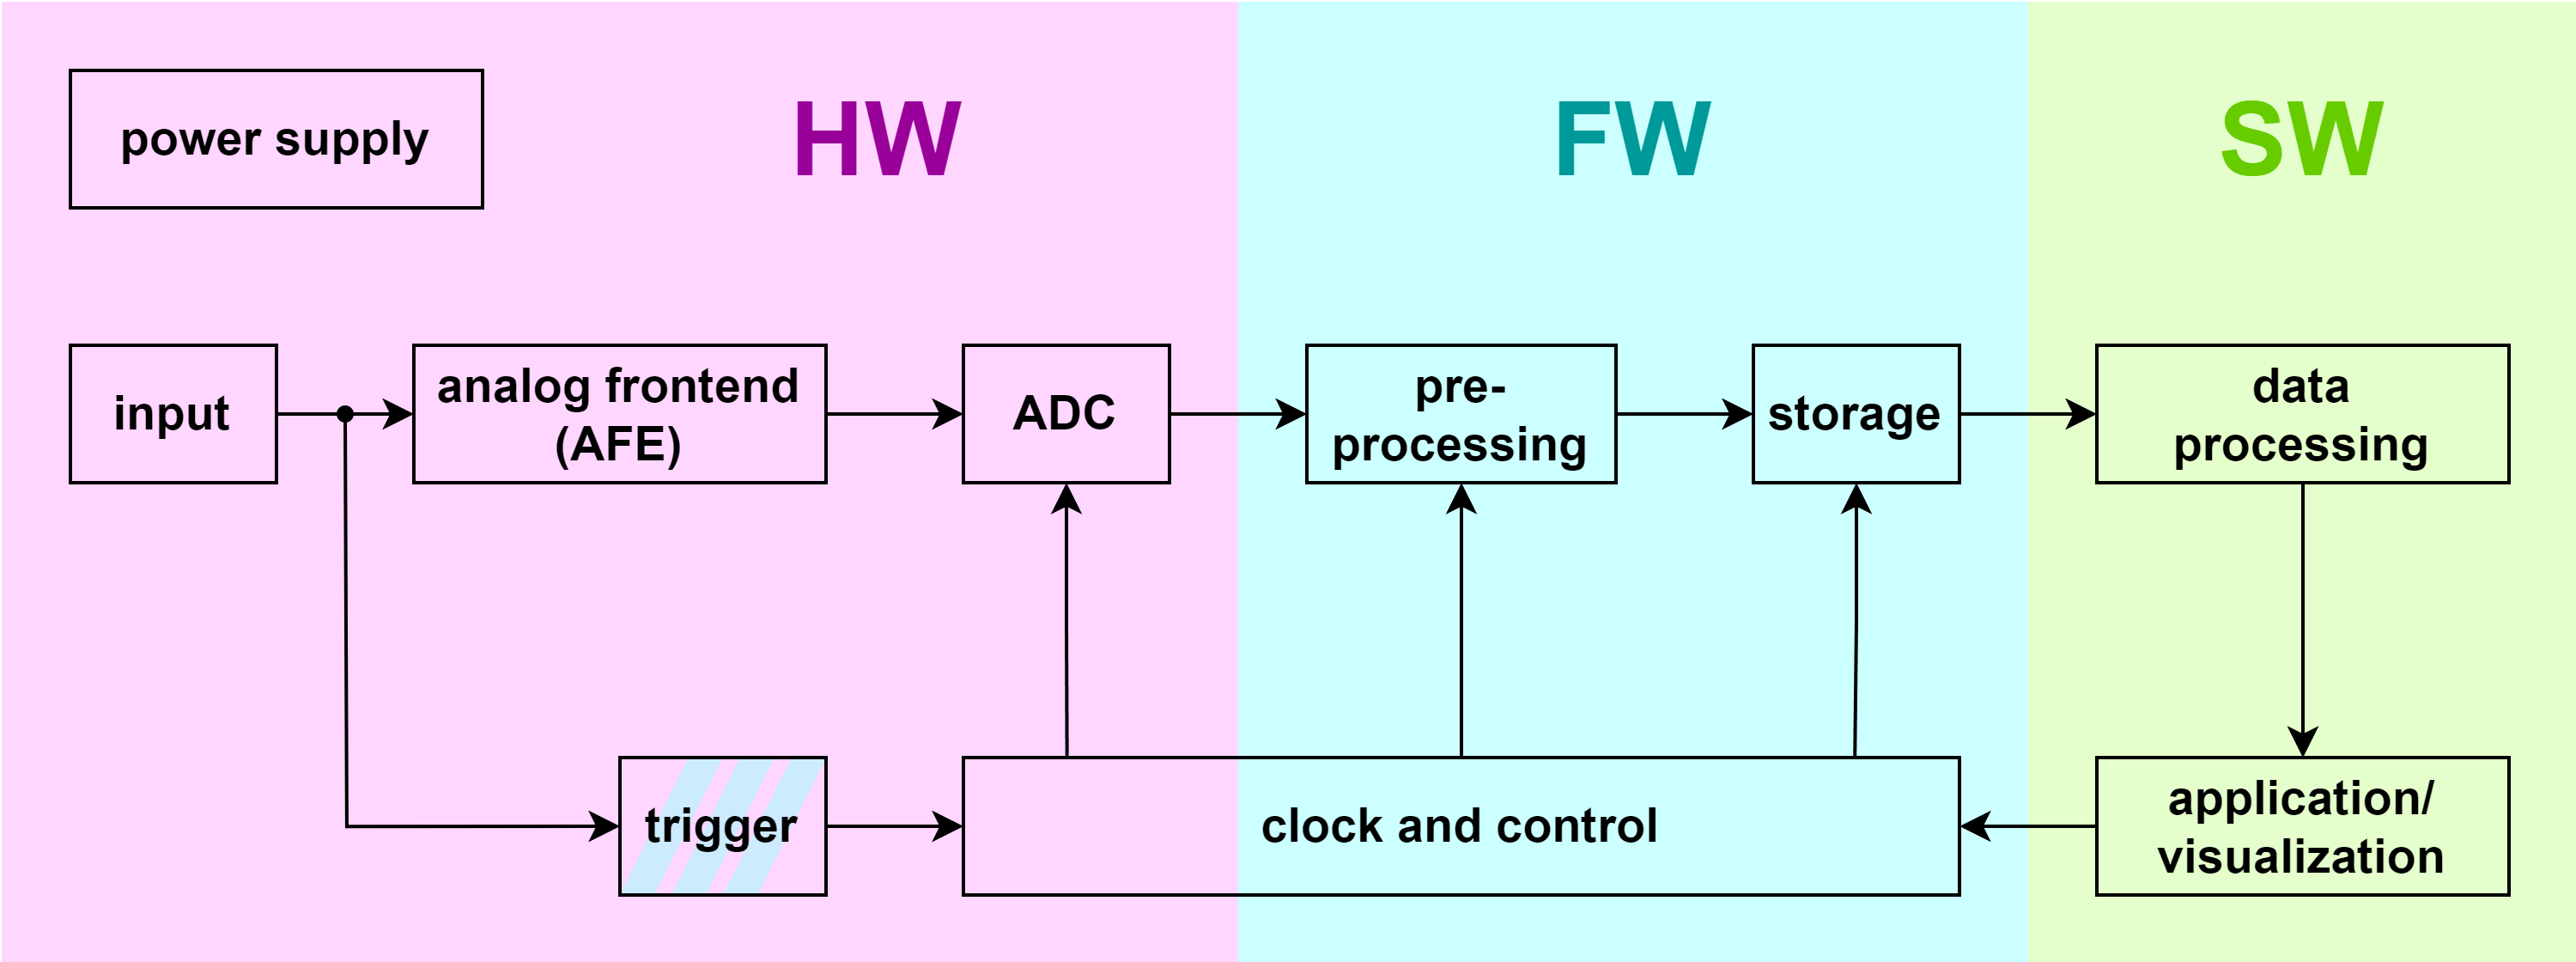
\includegraphics[scale=0.14]{Projektstruktur.png} 
	\caption{Gesamtkonzept des USB-Oszilloskops (nach \cite[S. 216]{Muehl2020})}
	\label{fig:complete_concept}
\end{figure}

Ausgehend von diesem Konzept und der klaren Aufteilung in die Bereiche Hardware, Firmware und Software, wurden die entsprechenden Schnittstellen festgelegt und die Aufgabenbereiche verteilt.

\pagebreak

%%%%%%%%%%% Realisierung %%%%%%%%%%%
\section{Realisierung}

\subsection{Hardware (HW)}
\subsubsection{Entwurf}
\subsubsection{Implementierung}
\subsubsection{HW-Test}

\subsection{Schnittstelle Hardware - Firmware}


\subsection{Firmware (FW)}
\subsubsection{Entwurf}
\subsubsection{Implementierung}
\subsubsection{FW-Test}

\subsection{Schnittstelle Firmware - Software}

\subsection{Software (SW)}

\subsection{Zusammenführung}
\subsubsection{Entwurf}
\subsubsection{Implementierung}
\subsubsection{SW-Test}

\pagebreak

%%%%%%%%%%% Schluss %%%%%%%%%

\pagebreak

%%%%%%%%%%% Ergebnisse %%%%%%%%%%%
\section{Ergebnisse}

\pagebreak

%%%%%%%%%%% Fazit und Ausblick %%%%%%%%%%%
\section{Fazit und Ausblick}

\pagebreak

%%%%%%%%%%% Literaturverzeichnis %%%%%%%%%%%
\section{Literaturverzeichnis}
\printbibliography
\pagebreak

%%%%%%%%%%% Abbildungsverzeichnis %%%%%%%%%%%
\section{Abbildungsverzeichnis}
\listoffigures
\pagebreak

%%%%%%%%%%% Abkürzungsverzeichnis %%%%%%%%%%%
%\section{Abkürungsverzeichnis}

%\begin{acronym}
%\acro{Abk.}{Abkürzung} % Im Text mit \ac{Abk.} verwenden
%\end{acronym}

%\pagebreak

%%%%%%%%%%% Anhang %%%%%%%%%%%
\appendix
\section{Anhang}
\label{sec:appendix_a}

  
\end{document}
